\documentclass[letterpaper]{article}

\usepackage{graphicx}  %Required
\usepackage{amsmath,amsfonts,amssymb}

\title{Supplementary Material:\\Disentangled Representation Learning for Non-Parallel Text Style Transfer}


\date{}
\author{}
\begin{document}
\maketitle
\graphicspath{{images/}}

\newcommand{\loss}[1]{J_{\text{#1}}}


\begin{figure}[ht!]
	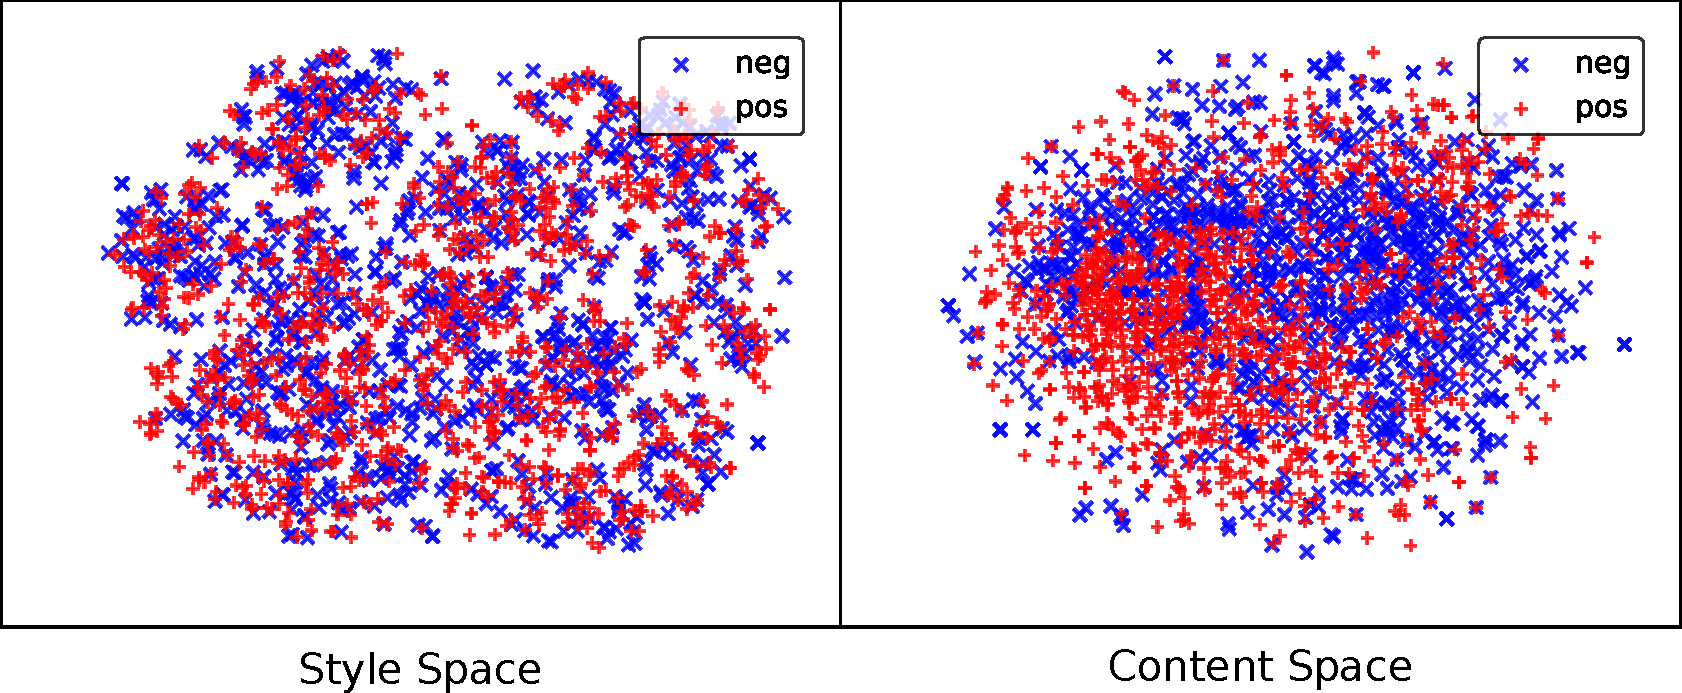
\includegraphics[width=\linewidth]{vae-latent-spaces-only-rec}
	\caption{t-SNE Plots: VAE with only $\loss{AE}$}
	\label{fig:vae-tsne-only-rec}
\end{figure}

\begin{figure}[ht!]
	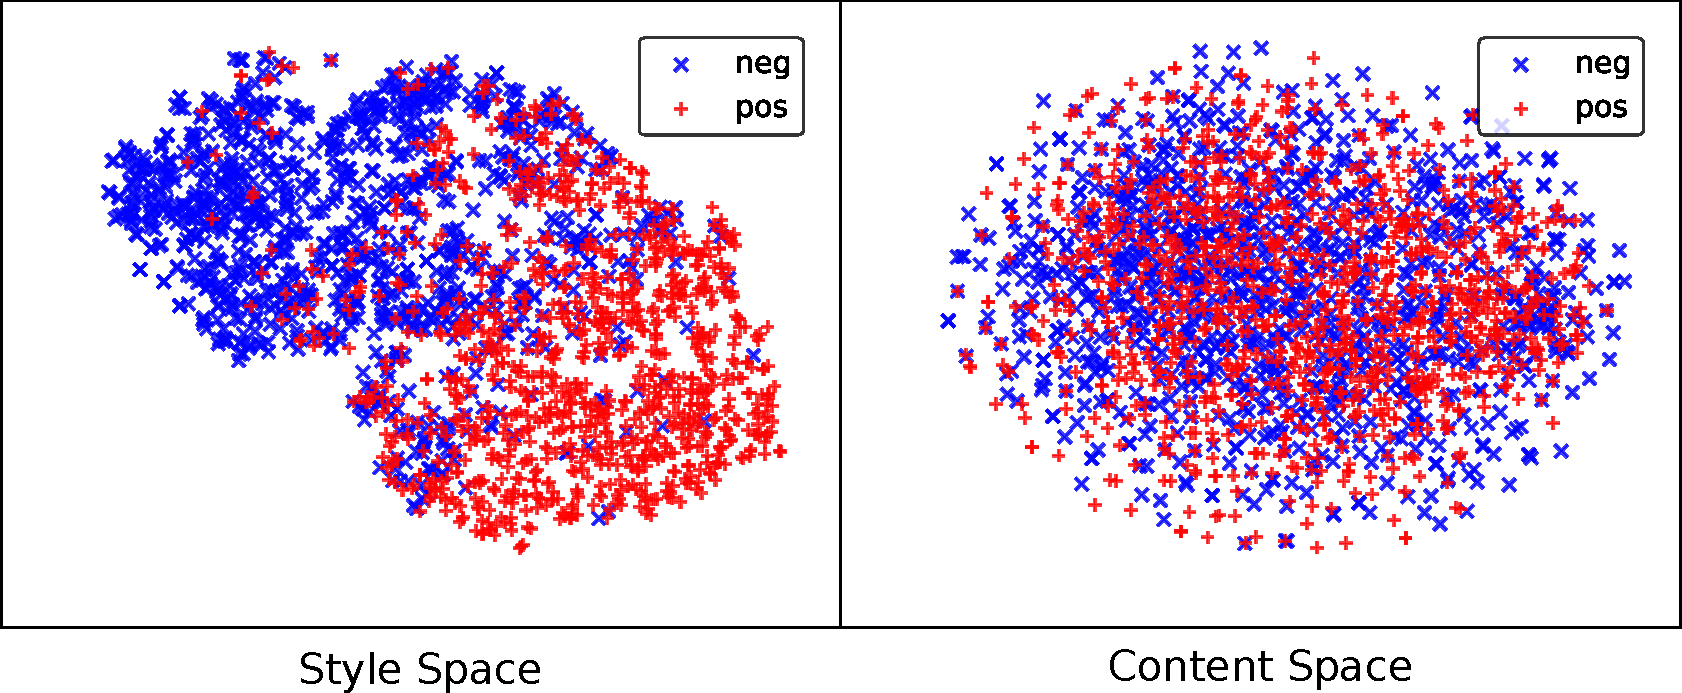
\includegraphics[width=\linewidth]{vae-latent-spaces-rec-adv}
	\caption{t-SNE Plots: VAE with $\loss{AE} + \loss{adv(s)}$}
	\label{fig:vae-tsne-rec-adv}
\end{figure}

\begin{figure}[ht!]
	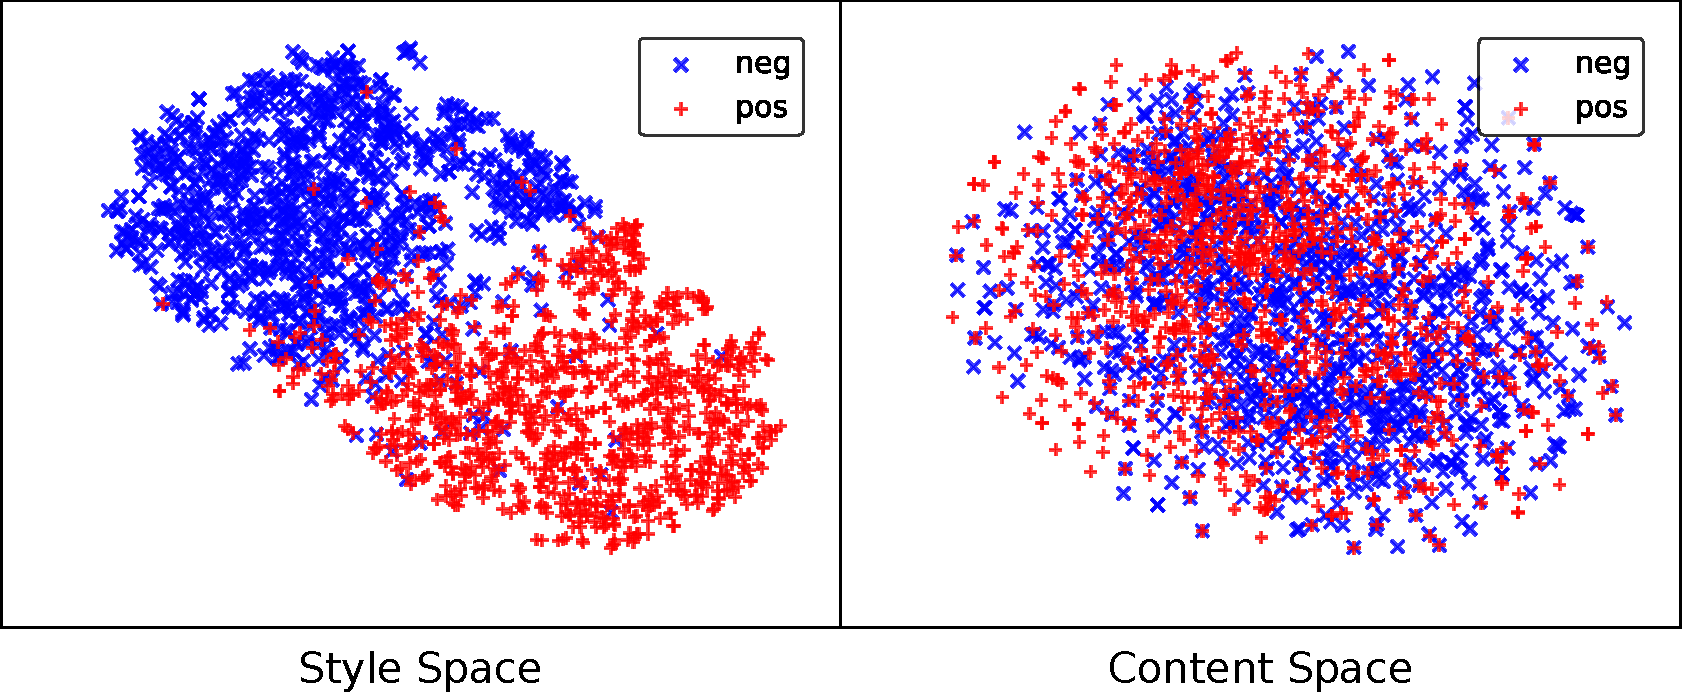
\includegraphics[width=\linewidth]{vae-latent-spaces-rec-mult}
	\caption{t-SNE Plots: VAE with $\loss{AE} + \loss{mul(s)}$}
	\label{fig:vae-tsne-rec-mult}
\end{figure}

\end{document}
